\documentclass[final,1p,times]{elsarticle}

\usepackage{amssymb}
\usepackage{amsmath,amsfonts}
\usepackage{algorithmic}
\usepackage{algorithm}
\usepackage{color,array}
\usepackage[caption=false,font=normalsize,labelfont=sf,textfont=sf]{subfig}
\usepackage{textcomp}
\usepackage{stfloats}
\usepackage{url}
\usepackage{verbatim}
\usepackage{graphics}
\usepackage{multirow}
\usepackage{bm}
\usepackage{threeparttable}
\usepackage{booktabs}
\usepackage{subfloat}

\renewcommand{\algorithmicrequire}{\textbf{Input:}}  
\renewcommand{\algorithmicensure}{\textbf{Output:}}
\newtheorem{myDef}{Definition}

%\journal{Expert Systems With Applications}

\bibliographystyle{model5-names}\biboptions{authoryear}

\begin{document}
	
\begin{frontmatter}
		
\title{Time-controlled incentive federated crowdsourcing}
		

\author[mymainaddress]{Xiaoqian Jiang }
\ead{220224926@seu.edu.cn}
		
\author[mymainaddress]{Jing Zhang
\corref{mycorrespondingauthor}}
\ead{jingz@seu.edu.cn}
		
%\author[thirdaddress]{}
%\ead{}
		
\cortext[mycorrespondingauthor]{Corresponding author}
\address[mymainaddress]{School of Cyber Science and Engineering, Southeast University, No. 2 SEU Road, Nanjing 211189, China}
%\address[thirdaddress]{}
		
\begin{abstract}
			
\end{abstract}
\begin{keyword}
	
\end{keyword}
\end{frontmatter}

\section{Introduction}
Crowdsourcing provides a feasible way to introduce human intelligence to solve notoriously difficult tasks that cannot be solved by computers alone \citep{Vaughan2017MakingBU}. One of the most widespread applications of crowdsourcing is to collect data from massive Internet workers. The collected data including annotations, locations, content, and so on could be further utilized in downstream AI tasks such as building CV \citep{Kovashka2016CrowdsourcingIC}, NLP \citep{Wang2013PerspectivesOC}, recommendation \citep{Lin2023CompetitiveGI} models. Commercial crowdsourcing platforms such as MTurk, Appen, etc., have provided effective interaction modes between task publishers and workers to facilitate the execution of crowdsourced tasks. It is worth noting that while crowdsourcing provides convenience, it may also expose workers' privacy, which will reduce workers' willingness to participate in tasks. Prior research has shown that sensitive private information such as behavior traits, vocal prints, face images, and locations could be revealed along with the submitted data \citep{xia2020privacy,Tong2020FederatedLI}. Thus, privacy issues are attracting more and more attention in crowdsourcing task design. Some traditional approaches can achieve privacy protection by adding perturbation (e.g., implemented as differential privacy \citep{luo2016incentive,wang2022pps}) or noises \citep{to2018ppo,huang2020traffic}. Notwithstanding, these methods undermine the quality of crowdsourcing since the data uploaded by the workers are blurred.

Crowdsourcing platforms are the hubs for collecting data uploaded by workers. Thus, they are key parts of privacy security, where privacy leaks will affect massive crowdsourcing workers. In current crowdsourcing applications, there is a large class of tasks that collect data (usually annotations) from workers and use them in subsequent machine learning processes \citep{Sheng2019MachineLW}. With the increasing computation power of end devices and the fast growth of broadband networks, the model building can be directly performed on the end devices instead of being processed on the platform. That is, we can introduce federated learning (FL) \citep{mcmahan2017communication} to perform learning tasks. FL allows multiple distributed clients to collaborate on training shared models by iteratively aggregating model updates without exposing the raw data, which realizes privacy-preserving model training with little performance loss \citep{Yang2019FederatedML,Gao2022ASO}. Currently, FL has been fused with crowdsourcing and performs well in some situations \citep{Pandey2019ACF,Tong2020FederatedLI,zhang2021enabling}.

Although FL can effectively mitigate privacy breaches in crowdsourcing it also requires clients (i.e., workers in crowdsourcing) to contribute their data, computing, and communications resources, involving considerable costs. On the other hand, processing data locally on the client side indeed protects privacy. However, malicious attackers and the curious server still exist, who always struggle to probe the privacy lying the training samples from intermediate model parameters and gradients \citep{lyu2020threats,Song2020AnalyzingUP}. Such anxiety toward privacy security exacerbates participant inertia in FL \citep{mothukuri2021survey}. In addition, clients in FL have absolute control over their own devices, bandwidth, and data. That is, only the owners of clients can decide when, where, and how to participate in FL \citep{Liu2021FromDM}. Therefore, the incentive mechanism is very important for clients to participate in FL efficiently \citep{zhan2021incentive}. Unless clients can obtain enough compensation, they are unwilling to take those risks and contribute their resources. Sufficient incentives will encourage clients to respond optimally and eventually improve the performance of learned models.

Current incentive mechanisms in FL are usually designed around the driving factors of clients’ contribution, reputation, and resource allocation \citep{zhan2020learning,zhan2021survey}. Those incentive mechanisms designed for FL, targeting addressing the problems of how to accurately measure the contribution of each client and how to effectively attract and retain more clients, do not work well in crowdsourcing scenarios. The reasons are as follows: \lowercase{\romannumeral1}) In federated crowdsourcing, clients (workers) usually have the right to choose the human-intelligence tasks that are suitable for them. Thus, the incentive mechanism also needs to mobilize workers' interest and enthusiasm for crowdsourcing tasks. For example, it encourages clients to contribute more fresh data/models to keep the global model updated. \lowercase{\romannumeral2}) Due to the heterogeneity of clients' objective environments (e.g., computation ability of devices, communication bandwidth, and data resources) and subjective environments (e.g., expertise, dedication, and intention of workers), time control should be considered in federated crowdsourcing. On the one hand, the process of federated crowdsourcing is not necessarily as fast as possible. Platforms need time to assess the quality of submitted outcomes to prevent malicious workers from submitting low-quality data/model for quick rewards. On the other hand, the server (task publisher) must efficiently respond to delays in receiving data due to device and network failures as well as worker disruptions on client ends rather than waiting passively. \lowercase{\romannumeral3}) In federal crowdsourcing, platforms need to recruit and retain high-quality workers. Workers (clients) expect to be paid fairly and as high as possible. Task publishers (servers) expect to obtain as many high-quality outcomes as possible within their budget. Thus, the incentive mechanism of federated crowdsourcing must make a trade-off among these factors.

To address the above challenges, this paper puts forward \underline{Ti}me-controlled incentive \underline{Fed}erated \underline{Crowd}sourcing (TiFedCrowd), which inspires clients to complete data collection and local model training within the given time limit to optimize the global learning model. TiFedCrowd models the federated crowdsourcing process as a two-stage Stackelberg game \citep{li2017review} with a time limit. In the second stage (rewarding clients), TiFedCrowd allots rewards to clients based on their local model accuracies. Here, only the clients that upload models within the given time will be accepted and rewarded. Clients will adjust their model accuracies in the next round according to the costs of completing federated crowdsourcing tasks (mainly including the computing and communication costs) and the rewards obtained from the server. Through this adjustment, clients will be more proactive in taking on crowdsourcing tasks. In the first stage (maximizing the net utility of the server), TiFedCrowd sets a time interval on the server side to ensure the quality and efficiency of the server-side trained global model while maximizing the server-side net utility. The net utility is defined as the profit obtained by training the global model minus the total cost of incentivizing clients. In addition, only the models uploaded by the clients within the given time interval will be accepted and rewarded. Finally, we derive the Nash equilibrium in the Stackelberg game, which describes the steady state of the federated crowdsourcing process. The main contributions of the paper are as follows: 

\begin{itemize}
	\item We propose a novel time-controlled incentive federated crowdsourcing (TiFedCrowd), which encourages more workers to complete crowdsourcing tasks with high quality and efficiency as well as protects the privacy of participants. A time interval is set to preliminarily screen the quality of submitted outcomes. The upper bound of the interval enables the publisher (server-side) to specify the fresh level of the submissions, which is applicable to both instant and non-instant crowdsourcing.
	\item The Nash equilibrium of the Stackelberg game is derived. We prove that the Nash equilibrium of the proposed method can reach a  global maximization of the server and the client utilities. Furthermore, we prove the time interval theoretically improves the utility of the server and the performance of the global model.
	\item TiFedCrowd allocates rewards according to contributions, which has strong interpretability. It is conducive to attracting and retaining high-quality crowdsourcing workers, thus maintaining the fairness and accountability of the federated crowdsourcing market.
\end{itemize}

The remainder of the paper is organized as follows: Section~\ref{sec:rw} briefly reviews the related studies.  Section~\ref{sec:mtd} presents the details of the proposed method.  Section~\ref{sec:exp} shows the experimental results and discusses them. Section~\ref{sec:con} concludes the paper with future work.

\section{Related Work}\label{sec:rw}
In this section, we briefly review the technical progress in two directions, i.e., privacy protection in crowdsourcing and incentive mechanism in federated learning.

\subsection{Privacy Protection in Crowdsourcing}
Since crowdsourcing usually involves collecting data from workers, it is inevitable that some tasks may touch workers' sensitive information. Thus, crowd workers face the risk of privacy disclosure \citep{xu2019blockchain,zhang2020decentralized}. Although differential privacy \citep{dwork2006differential} has been widely favored in the research field of Internet privacy protection since it was proposed, it works by injecting different levels of noise into the model. Undoubtedly, differential privacy will more or less sacrifice the accuracy of models \citep{bagdasaryan2019differential}. In addition, there are also techniques to protect the privacy of crowd workers that introduce various cryptographic algorithms. For example, \cite{shu2018privacy} proposed a privacy-preserving task recommendation scheme for crowdsourcing, which exploits polynomial functions to express multiple keywords of task requirements and worker interests, and then designed a key derivation method based on matrix decomposition. \cite{joshi2020salt} used SALT cryptography in the proposed solution to ensure privacy. \cite{zhang2019privacy} proposed a privacy-preserving traffic monitoring scheme through both adopting a homomorphic Paillier cryptosystem and super-increasing sequence. However, These encryption algorithms are complex, expensive, and cannot resist inference attacks \citep{lin2020secbcs,wang2019towards}.

To overcome the above defects, researchers introduced federated learning, which provides a secure way to work together so that participants can share and leverage data without exposing their privacy. For example, mean teacher semi-supervised FL \citep{zhang2021toward} introduces FL to provide a privacy-preserving framework for deep learning to realize the benefits of crowdsourcing. \cite{li2020crowdsf} proposed a crowdsourcing framework named CrowdSFL, which combines blockchain with FL to help users implement crowdsourcing with less overhead and higher security. These approaches to privacy protection in crowdsourcing by introducing the FL framework are all based on the ideal condition that participants are fully willing to make any contribution. However, FL usually requires considerable costs on the client's end. In most cases, crowd workers do not have such passions to contribute without enough rewards.

\subsection{Incentive Mechanism in Federated Learning}
An incentive mechanism is necessary to ensure the quality and efficiency of FL. The participation of clients in FL consumes computing resources, occupies network bandwidth, and even shortens the battery life of client devices. Clients are not willing to make sacrifices to participate in FL without any return. Accordingly, there is a growing body of research on the incentive mechanism of FL. \cite{zhan2020learn} designed a deep reinforcement learning-based incentive mechanism to determine the optimal pricing strategy for the parameter server and the optimal training strategies for edge nodes. \cite{le2021incentive} formulated the incentive mechanism between the base station and mobile users as an auction game and further proposed the primal-dual greedy auction mechanism to decide winners in the auction and maximize social welfare. \cite{zhang2021incentive} proposed an incentive mechanism of FL based on reputation and reverse auction theory, which selects and rewards participants by combining the reputation and bids of the participants under a limited budget.  \cite{9317806} modeled each data owner's contribution and the three categories of computing, communication, and privacy costs based on a multi-dimensional contract approach. \cite{pandey2019incentivize} introduced the crowdsourcing framework into FL and developed a two-stage Starkelberg game to maintain communication efficiency when participating clients implement uncoordinated computation strategy during aggregation of model parameters. \cite{kang2022incentive} proposed the incentive-boosted Federated Crowdsourcing and modeled the incentive-based interaction between the crowdsourcing platform and participating workers as a Stackelberg game to encourage workers to constantly collect fresh data.

Unfortunately, none of these incentive mechanisms works well in federated crowdsourcing that needs to collect data samples manually (i.e., so-call data crowdsourcing). Moreover, they all ignore the relationship between the time that workers collect data and the quality of submitted data in federated crowdsourcing and fail to respond to some delays in receiving data. The proposed TiFedCrowd in this study sets a time interval whose lower bound preliminarily screens the quality of submitted data and whose upper bound enables the task publisher to specify the fresh level of the data. Furthermore, the contribution of a worker is measured according to the accuracy \footnote{In this study, we simply use accuracy to measure the performance of learning models.} with which the client completes a local training model within the given time, and the rewards are fairly allocated in an economical manner, so as to motivate more workers to complete crowdsourcing tasks with high quality and efficiency.

\section{Methodology} \label{sec:mtd}
In this section, we first present the federated crowdsourcing problem settings. Then, we present the proposed incentive mechanism as a two-stage Stackelberg game and also derive its equilibrium. Next, we summarize the whole process as an algorithm. Finally, we prove that time control is necessary for federated crowdsourcing.

\begin{figure}
	\centering
	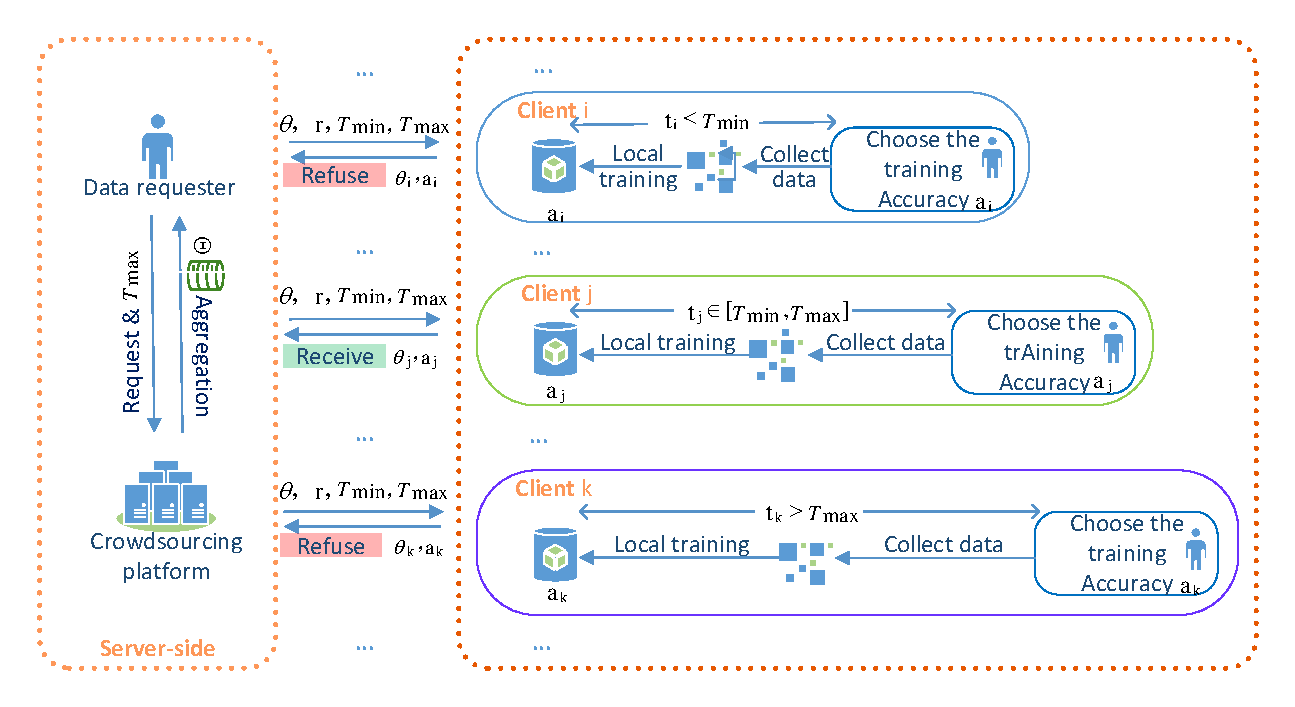
\includegraphics[width=5.5in]{TiFedCrowd framework.pdf}
	\caption{Framework of the time-controlled incentive federated crowdsourcing (TiFedCrowd).}
	\label{fig:framework}
\end{figure}

\subsection{Problem Settings}
Let $\bm{\mathcal{N}} = \{1,2,\dots,n\}$ be a group of workers participating in federated crowdsourcing. For each worker $k\in\bm{\mathcal{N}}$, let $D_k=\{\bm{x_i}^k,y_i^k\}_{i=1}^m$ be the data sample set, where $m$ is the number of tasks, $\bm{x_i}^k\in\mathbb{R}^d$ is a vector with $d$ features representing the task for annotation, and $y_i^k\in\mathbb{R}$ is the label annotated for task $\bm{x_i}^k$ by worker $k$. To achieve privacy protection, TiFedCrowd requires that $D_k$ be kept locally and not shared with the server or other clients. In addition, each client trains its own local model $\theta_k$ through $D_k$ to collaboratively train the shared model $\Theta$.

Figure~\ref{fig:framework} shows the framework of the proposed TiFedCrowd model. The data requester first publishes task requirements and the allowed maximum completion time $T_{\max}$ through a crowdsourcing platform. Then, the platform (server) calculates the allowed minimum completion time $T_{\min}$ by evaluating task difficulty level and network quality and announces it to all clients along with the to-be-trained model $\theta$ and the reward rate $r$. For any client $k$, it determines his/her training accuracy level at the reward rate $r$. Next, the client collects data on demand to train the local model for attaining accuracy $a_k^\ast$ and sends the updated model to the server. Only those models uploaded within the time interval $[T_{\min},T_{\max}]$ will be accepted by the server, otherwise, they will be rejected. In this process, if the completion time of a model is greater than $T_{\max}$, it indicates that the local model updating may encounter some errors (i.e., network unavailable, training corrupt, data collection failed, etc.). The server will no longer receive the model. Another function of $T_{\max}$ is to control the fresh level of local models. The server will reject the local models whose completion times are greater than $T_{\max}$, deeming them outdated. If the completion time of a model is less than $T_{\min}$, it indicates that the client may not take the task seriously. The server also rejects it.  Finally, the server aggregates the received local models $\{\theta_k\}_{k=1}^n,T_k\in[T_{\min},T_{\max}]$ to obtain a global model and then distributes the rewards to clients whose models are successfully accepted according to the accuracy levels that they archived. 

The proposed TiFedCrowd aims to achieve a win-win situation using a novel incentive mechanism. Ideally, the server-side tries to encourage clients to contribute high-quality local models using as less as budget. whereas, the clients try to obtain more rewards by providing qualified outcomes within the specified time interval. Clearly, it is a gaming process. In the following sections, we will show that TiFedCrowd can reach an equilibrium status, where the utilities of both server and clients can be optimal. We will also show that introducing the time interval $[T_{\min}, T_{\max}]$ not only brings practical values (controlling the fresh levels of local models and filtering out low-quality local models) but also theoretically improves the utility of the server and the performance of the global model.

\subsection{Incentive Mechanism: The Two-Stage Stackelberg Game}
In the proposed time-controlled incentive federated crowdsourcing model, the data requester rewards clients who complete tasks within the specified time to achieve optimal local accuracy, thereby optimizing the global model. Simultaneously, upon receiving the rewards, rational clients will maximize their own profits respectively by improving the accuracy of the local models. We model such an interaction scenario as a two-stage Stackelberg game between a server (leader) and multiple clients (followers). In the Stackelberg game, both parties choose their own strategies based on the other's possible strategies to ensure that they maximize their interests under the other's strategy, so as to achieve the Nash equilibrium. The party that makes a decision first is called the leader. The remaining players (followers) make decisions based on the leader's decision. Then, the leader and followers adjust the initial decisions to make final better decisions by predicting the other party's response to their own decisions. The process is repeated until reaching the Nash equilibrium. 

Under our problem settings, the server first publishes local model requirements. Then, in Stage \uppercase\expandafter{\romannumeral2}, each client individually determines his/her own training accuracy according to the announced reward to maximize profit. After clients submit their work outcomes. In stage \uppercase\expandafter{\romannumeral1}, the server decides on the reward rate for clients to maximize the net utility and train the high-quality global model.

\textbf{Stage \uppercase\expandafter{\romannumeral2} (Clients):} In the client stage, the server will initially announce the uniform reward rate $r>0$ and time interval $[T_{\min},T_{\max}]$ for the participating clients. Rationally, for a client $k$, the reward $v_k$ is related to the accuracy level $a_k$ of the local model $\theta_k$. Intuitively, the higher the local accuracy level, the greater the revenue is:
\begin{equation}\label{eq:reward}
	v_k = r\cdot a_k\cdot \mathbb{I}(\tau),
\end{equation}
where $\mathbb{I}(\tau)$ is an indicator function that returns $1$ if the condition $\tau$ is true and $0$ otherwise. Only if the completion time $T_k$ meets condition $\tau: T_k\in[T_{\min},T_{\max}]$ will the model $\theta_k$ be accepted by the server and the reward $v_k$ be allocated. We refer to clients whose models are successfully accepted by the server as valid participants. Then, a rational worker will try to collect data to train a local model with high accuracy within the time limit for maximization of the revenue.  

Obviously, it inevitably brings costs $c_k$ for client $k$ to train a local model with a pre-defined accuracy on local data that can improve the global model. The costs include the computation cost $c_k^{comp}$ and the communication cost $c_k^{comm}$. That is, 
\begin{equation}\label{eq:cost}
	c_k	= c_k^{comp} + c_k^{comm}.
\end{equation}
Here, $c_k$ can be treated as the total cost of client $k$'s participation. The computation cost $c_k^{comp}$ is relevant to the number of iterations for training the local model $\theta_k$ to the target accuracy $a_k$. According to the relationship between iterations and accuracy in the local model training described in \citep{pandey2020crowdsourcing}, the computation cost of client $k$ is defined as follows:
\begin{equation}
	c_k^{comp} = \gamma_k\cdot \log(\frac{1}{1-a_k}),
\end{equation}
where $\gamma_k>0$ is a parameter choice of client $k$ that depends on the data size and condition number of the local subproblem \citep{konevcny2017semi}. Therefore, the more iterations of the local model training, the more computing resources the client spends.

The communication cost is related to the size of the model parameters and is incurred when the client interacts with the server for the model update. Since the to-be-trained model is published uniformly by the server, the total communication cost is the same for all clients as follows:
\begin{equation}
	c_k^{comm} = \lambda\cdot\xi,
\end{equation}
where $\lambda$ is a constant coefficient and $\xi$ represents the size of the model parameter.

Combining reward in Eq. (\ref{eq:reward}) and cost in Eq. (\ref{eq:cost}) of the client, for a valid participant, we define the utility of a client as follows:
\begin{equation}\label{eq:client-u}
	u_k = r\cdot a_k - c_k, \quad only\,\: if\quad\mathbb{I}(\tau) = 1.
\end{equation}

\textbf{Stage \uppercase\expandafter{\romannumeral1} (Server):} In the server stage of the game, the server can evaluate the optimal reward rate $r^\ast$ to maximize its net utility according to the response of valid participants. Let $\zeta$ be the number of valid participants, i.e.,
\begin{equation}
	\zeta = \sum_{k=1}^n\mathbb{I}(\tau).
\end{equation}
The utility of the server can be defined in relation to the maximum completion time of valid participants and the performance of the final global model achieved based on average local accuracy level. That is, 
\begin{equation}\label{Eq:server-u}
	U = \frac{1}{\zeta}\cdot \sum_{k=1}^n\left(\alpha\cdot a_k\cdot \mathbb{I}(\tau)\right) + \beta\cdot(T_{\max}-\max_{\mathbb{I}(\tau)=1,1\le k\le n}T_k) - \sum_{k=1}^n\left(r\cdot a_k\cdot \mathbb{I}(\tau)\right),
\end{equation}
where $\alpha > 0$ and $\beta \ge 0$ are system parameters, and $\sum_{k=1}^n(r\cdot a_k\cdot \mathbb{I}(\tau))$ is the cost totally spent for incentivizing clients that have validly participated in federated crowdsourcing. By default, we have $\beta = 0$, and $\beta > 0$ only makes sense in instant crowdsourcing (fresh data/model needs to be collected/trained constantly).

\subsection{Nash Equilibrium}
In this subsection, we will present the optimal solution to maximize the utility of both clients and the server by deducing the Nash equilibrium.

\begin{myDef}
	Nash Equilibrium. For any values of $r$ and $\bm{a}$, $(r^\ast,\bm{a}^\ast)$ is a Nash equilibrium if they satisfy the following conditions:
	\begin{equation}
		U(r^\ast,\bm{a}^\ast) \ge U(r,\bm{a}^\ast),
	\end{equation}	
	\begin{equation}
		u_k(r^\ast,a_k^\ast) \ge u_k(r^\ast,a_k),\, \forall k \in \bm{\mathcal{N}}.
	\end{equation}	
\end{myDef}

To find the equilibrium of the client stage in the game, we take the first derivative of $u_k(r,a_k)$ with respect to $a_k$ as follows:
\begin{equation}
	\frac{\partial u_k(r,a_k)}{\partial a_k} = r-\frac{\gamma_k}{1-a_k}.
\end{equation}	

Let $\frac{\partial u_k(r,a_k)}{\partial a_k} = 0$, we have
\begin{equation}\label{eq:a_k_ast}
	a_k^\ast = 1 - \frac{\gamma_k}{r}.
\end{equation}	

Then, we take the second derivative of $u_k(r,a_k)$ with respect to $a_k$ as follows:
\begin{equation}
	\frac{\partial^2 u_k(r,a_k)}{\partial a_k^2} = - \frac{\gamma_k}{(1-a_k)^2} < 0.
\end{equation}	

Hence, we derive and prove that $a_k^\ast = 1 - \frac{\gamma_k}{r}$ is the global optimal response accuracy of the client and is unique.

Since we have $0<a_k^\ast<1$, we can derive the value range of the reward rate $r$ as follows:
\begin{equation}
	0 < a_k^\ast = 1 - \frac{\gamma_k}{r} < 1\quad
	\Leftrightarrow\quad r > \gamma_k.
\end{equation}	

Based on the above derivations for clients (followers), as the leader in the game, the server can deduce the unique Nash equilibrium among valid participants for any reward rate $r>\gamma_k$. Accordingly, the server can choose the optimal reward rate $r^\ast$ to maximize its net utility. Based upon the sets of the completion time $\bm{T}^\ast$ and the optimum response accuracy $\bm{a}^\ast$, utility of the server is defined as follows:
\begin{equation}\label{eq:opt_u}
	U(r,\bm{a}^\ast) = \frac{1}{\zeta}\cdot \sum_{k=1}^n(\alpha\cdot a_k^\ast\cdot \mathbb{I}(\tau)) + \beta\cdot(T_{\max}-\max_{\mathbb{I}(\tau)=1,1\le k\le n}T_k^\ast) - \sum_{k=1}^n(r\cdot a_k^\ast\cdot \mathbb{I}(\tau)).
\end{equation}

Taking the first derivative of $U(r,\bm{a}^\ast)$ with respect to $r$, we obtain
\begin{equation}
		\begin{aligned}
		\frac{\partial U(r,\bm{a}^\ast)}{\partial r} &= \frac{1}{\zeta}\cdot \sum_{k=1}^n\left(\alpha\cdot \frac{\partial a_k^\ast}{\partial r}\cdot \mathbb{I}(\tau)\right) - \sum_{k=1}^n\left(r\cdot \frac{\partial a_k^\ast}{\partial r}\ast\cdot \mathbb{I}(\tau)\right) - \sum_{k=1}^n(a_k^\ast\cdot \mathbb{I}(\tau))\\&= \frac{\alpha}{\zeta\cdot r^2}\cdot\sum_{k=1}^n(\gamma_k\cdot\mathbb{I}(\tau))-\zeta.
	\end{aligned}
\end{equation}

Let $\frac{\partial U(r,\bm{a}^\ast)}{\partial r} = 0$, we have
\begin{equation}\label{eq:opt_r}
	r^\ast =\frac{1}{\zeta}\cdot\sqrt{\alpha\cdot\sum_{k=1}^n(\gamma_k\cdot\mathbb{I}(\tau))}.
\end{equation}	

The second derivative of $u_k(r,a_k)$ with respect to $r$ is as follows
\begin{equation}
	\frac{\partial^2 U(r,\bm{a}^\ast)}{\partial r^2} = - \frac{2\cdot\alpha}{\zeta\cdot r^3}\cdot\sum_{k=1}^n(\gamma_k\cdot\mathbb{I}(\tau)) < 0.
\end{equation}	

Therefore, we have proved that $r^\ast = \frac{1}{\zeta}\cdot\sqrt{\alpha\cdot\sum_{k=1}^n(\gamma_k\cdot\mathbb{I}(\tau))}$ is the global optimal reward rate and it is unique. 

To sum up, we have found the unique Nash equilibrium of the proposed incentive mechanism under federated crowdsourcing.

\subsection{Why Time Control Important}
To ensure the quality and efficiency of crowdsourcing, TiFedCrowd limits the time for the clients to complete the federated crowdsourcing tasks by setting a time interval $[T_{\min},T_{\max}]$. The upper bound $T_{\max}$ is set by the data/model requester according to his/her needs. $T_{\max}$ can make the server timely respond to the delays in receiving data which resulted from device and network failures as well as disruptions on clients rather than waiting passively. In addition, the completion deadline $T_{\max}$ also indicates the requester's recognition of the freshness of the data/models. In other words, as long as the data/models are submitted before $T_{\max}$, they are considered fresh. In addition, the completion deadline $T_{\max}$ also indicates the data requester's recognition of the freshness of the data. In other words, as long as the data submitted before $T_{\max}$ is considered fresh. The lower bound $T_{\min}$ is calculated by the server based on the task difficulty and network quality, which prevents malicious clients from submitting low-quality data/model for quick rewards. The ultimate goal of TiFedCrowd is to obtain a high-quality global model, based on which we demonstrate that time control is necessary for federal crowdsourcing.

Based on Eq.~(\ref{Eq:server-u}), we remove the time control in the definition of the server utility as follows: 
\begin{equation}
	\bar{U} = \frac{1}{n}\cdot \sum_{k=1}^n(\alpha\cdot a_k)  - \sum_{k=1}^n(r\cdot a_k),
\end{equation}
where $\sum_{k=1}^n(r\cdot a_k)$ is the cost totally spent for incentivizing clients to participate in federated crowdsourcing. Apparently, the total cost $\sum_{k=1}^n(r\cdot a_k)$ for the server without time control is more than $\sum_{k=1}^n(r\cdot a_k\cdot \mathbb{I}(\tau))$ for one with time control.

To compare the magnitude of $\bar{U}$ and $U$, we take the difference between $\bar{U}$ and $U$:
\begin{equation}
	\bar{U} -U = \frac{1}{n}\cdot \sum_{k=1}^n(\alpha\cdot a_k)-\frac{1}{\zeta}\cdot \sum_{k=1}^n(\alpha\cdot a_k\cdot \mathbb{I}(\tau))- \beta\cdot(T_{\max}-\max_{\mathbb{I}(\tau)=1,1\le k\le n}T_k) - \sum_{k=1}^n(r\cdot a_k\cdot (1-\mathbb{I}(\tau))).
\end{equation}

For those data/models submitted after the deadline $T_{\max}$, whose freshness does not meet the requirements of the requester, we consider the accuracy level of their contributions to be $0$. Since TiFedCrowd uses the time control mechanism to filter out low-quality data/models, we have the following results:
\begin{equation}
	\begin{aligned}
		\frac{1}{n}\cdot \sum_{k=1}^n a_k < \frac{1}{\zeta}\cdot \sum_{k=1}^n a_k\cdot \mathbb{I}(\tau)\quad
		&\Leftrightarrow\quad \frac{1}{n}\cdot \sum_{k=1}^n(\alpha\cdot a_k)-\frac{1}{\zeta}\cdot \sum_{k=1}^n(\alpha\cdot a_k\cdot \mathbb{I}(\tau))<0\\&\Leftrightarrow\quad  \bar{U} -U<0\quad\Leftrightarrow\quad  \bar{U} < U.
	\end{aligned}
\end{equation}	

In summary, we show that the server without time control has less utility and more incentivizing cost than the one with it. consequently, time control is critical to federated crowdsourcing.

\subsection{Algorithm}
The pseudo-code of TiFedCrowd is shown in Algorithm~\ref{Algo1}. Lines 2-13 are the procedures on the server side and lines 15-19 are for clients. Precisely, the process of the server side includes the following four steps: 1) estimate the minimum completion time (line 2); 2) calculate the optimum response accuracy at the given reward rate for each valid participant (lines 3-8); 3) computing the optimum reward rate, and announce it to clients, then wait until the deadline for them to complete the tasks (lines 10-12); 4) receive the updated models and return the aggregated global model (line 13).

The process of the client side includes the following three steps: 1) receive the task completion time interval and the declared reward rate from the server (line 15); 2) determine the optimum model accuracy and train a local model to achieve the accuracy within the specified time interval (lines 17-18); 3) send the trained local model to the server (line 19).

\begin{algorithm}[H]
	\caption{\underline {Ti}me-controlled incentive \underline{Fed}erated \underline{Crowd}sourcing (TiFedCrowd)}
	\label{Algo1}
	\begin{algorithmic}[1]
		\REQUIRE clients $\bm{\mathcal{N}} = \{1,2,\dots,n\}$; local data sample sets $\{D_k\}_{k=1}^n$; computation
		parameters $\{\gamma_k\}_{k=1}^n$; size of the published model $\xi$;  system parameters $\alpha$ and $\beta$; completion deadline $T_{\max}$.
		\ENSURE global learning model $\Theta$.\\
		\COMMENT{\textit{Procedure at the server}}
		\STATE Sever initializes the system parameters $\alpha$ and $\beta$ by the task type.
		\STATE Estimate the minimum completion time $T_{\min}$.
		\FOR{all clients $k = 1 \to n$ in parallel}
		\IF {completion time $T_k\in[T_{\min},T_{\max}]$}
		\STATE Compute the client $k$’s utility $u_k$ at the given reward rates $r$ via Eq. (\ref{eq:client-u}).
		\STATE Calculate the optimal response accuracy $a_k^\ast$ via Eq. (\ref{eq:a_k_ast}).
		\ENDIF
		\ENDFOR
		\STATE Compute the server’s utility via Eq. (\ref{eq:opt_u}).
		\STATE Choose the optimum reward rate $r^\ast$ via Eq. (\ref{eq:opt_r}), then announce it to all clients.
		\STATE Wait until time $T_{\max}$ for clients to complete the data collection and model training.
		\STATE Receive the updated models $\{\theta_k\}_{k=1}^n$ and send the rewards to valid participants based on their accuracy levels. Aggregate the global model $\Theta$.
		\RETURN the global model $\Theta$.\\
		\COMMENT{\textit{Procedure at client $k$}}
		\STATE Client initializes the computation
		parameter $\gamma_k$ according to the data size and condition number of the local subproblem.
		\STATE Receive the time interval $[T_{\min},T_{\max}]$ and the reward rate $r$.
		\STATE Compute the client utility $u_k$ via Eq. (\ref{eq:client-u}).
		\STATE Determine the training accuracy $a_k^\ast$ to solve the local subproblem via Eq. (\ref{eq:a_k_ast}).
		\STATE Collect the required data and train local model for attaining the accuracy level $a_k^\ast$ within the time interval $[T_{\min},T_{\max}]$.
		\RETURN the trained local model $\theta_k$ to the server.
	\end{algorithmic}
\end{algorithm}

The time complexity analysis of this algorithm needs to be discussed from the client side and the server side respectively. On the client side, the main time consumption of the algorithm is data collection and model training. The data collection time complexity is $O(m)$, where $m$ is the number of tasks collected by the client. The model training time complexity is $O(\log(a_k^{-1}))$, related to training the local model for attaining the accuracy $a_k$. Hence, the total time complexity of TiFedCrowd on the client side is $S[O(m)+O(\log(a_k^{-1}))]$. The space complexity is $O(\xi)$, where $\xi$ is the size of model parameters. On the server side, the main time consumption is to interact with the $n$ clients and the main space consumption is to aggregate the $n$ client models. Therefore, the time complexity of TiFedCrowd on the server side is $O(n)$ and the space complexity is $O(n\cdot\xi)$.

\section{TiFedCrowd at Multiple Heterogeneous Federated Crowdsourcing Tasks}
In this section, we discuss how TiFedCrowd works in the case of heterogeneous federated crowdsourced tasks. Specifically, this is the extension of TiFedCrowd to publish multiple federated crowdsourced tasks simultaneously. 
\subsection{Problem Settings}
Let $\{\Omega^{(i)}\}_{i=1}^s$ be a heterogeneous set of federated crowdsourcing tasks and $s$ indicates the number of types of tasks. The data requester first publishes task requirements and the uniform allowed maximum completion time $T_{\max}$. Let $\{\bm{\mathcal{N}}^{(i)}\}_{i=1}^s$ be $s$ groups of workers participating in the tasks and $\bm{\mathcal{N}}^{(i)} = \{1^{(i)},2^{(i)},\dots,n^{(i)}\}$ ($n^{(i)}$ is the number of workers involved in task $\Omega^{(i)}$.). The server calculates the minimum completion time $\{T_{\min}^{(i)}\}_{i=1}^s$ by evaluating the difficulty of the different types of tasks and combining the network quality and then announces them to all clients along with the to-be-trained model $\{\theta^{(i)}\}_{i=1}^s$ and the reward rates $\{r^{(i)}\}_{i=1}^s$. The reward rate $r^{(i)}$ varies by the type of task $\Omega^{(i)}$ to prevent clients from selecting only simple tasks and let $\{\xi^{(i)}\}_{i=1}^s$ be the size of the parameters of these models. 
\subsection{The Two-Stage Stackelberg Game}
The clients stage: A client $k^{(i)}\in\bm{\mathcal{N}}^{(i)}\subseteq\{\bm{\mathcal{N}}^{(i)}\}_{i=1}^s$ tries to collect data on demand to train the local model for attaining accuracy ${a_k^{(i)}}^\ast$ and sends the updated model $\theta_k^{(i)}$ to the server within the time interval $[T_{\min}^{(i)},T_{\max}]$ to collaboratively train the shared model $\Theta$. Therefore, for a valid participant whose completion time $T_k^{(i)}$ meets condition $\tau^{(i)}:T_k^{(i)}\in[T_{\min}^{(i)},T_{\max}]$, we define the utility of a client as follows:
\begin{equation}
	u_k^{(i)} = r^{(i)}\cdot a_k^{(i)} - c_k^{(i)}, \quad only\,\: if\quad\mathbb{I}(\tau^{(i)}) = 1.
\end{equation}
Here $c_k^{(i)}$ is the total cost of client $k^{(i)}$'s participation:
\begin{equation}
	c_k^{(i)} = \gamma_k^{(i)}\cdot \log(\frac{1}{1-a_k^{(i)}})+\lambda\cdot\xi^{(i)},
\end{equation}
where $\gamma_k^{(i)}\cdot \log(\frac{1}{1-a_k^{(i)}})$ is the computation cost and $\lambda\cdot\xi^{(i)}$ is the communication cost.

The server stage: The utility of the server in TiFedCrowd at heterogeneous tasks is defined as follows:
\begin{equation}
	\mathcal{U} = \frac{1}{\zeta}\cdot \sum_{i=1}^{s}\sum_{k=1}^{n^{(i)}}\left(\alpha^{(i)}\cdot a_k^{(i)}\cdot \mathbb{I}(\tau^{(i)})\right) + \beta\cdot(T_{\max}-\max_{\mathbb{I}(\tau^{(i)})=1,1\le k\le n^{(i)},1\le i\le s}T_k^{(i)}) - \sum_{i=1}^{s}\sum_{k=1}^{n^{(i)}}\left(r^{(i)}\cdot a_k^{(i)}\cdot \mathbb{I}(\tau^{(i)})\right),
\end{equation}
where the system parameters $\{\alpha^{(i)}\}_{i=1}^s$ ($\alpha^{(i)}>0$) can also represent the weight of heterogeneous tasks and $\sum_{i=1}^{s}\sum_{k=1}^{n^{(i)}}\left(r^{(i)}\cdot a_k^{(i)}\cdot \mathbb{I}(\tau^{(i)})\right)$ is the cost totally spent for incentivizing clients that have validly participated in federated crowdsourcing. In addition, the number of valid participants $\zeta$ is calculated as: 
\begin{equation}
	\zeta = \sum_{i=1}^{s}\sum_{k=1}^{n^{(i)}}\mathbb{I}(\tau^{(i)}).
\end{equation}
\subsection{Nash Equilibrium for Heterogeneous Tasks in TiFedCrowd}
\begin{myDef}
	Nash Equilibrium for Heterogeneous Tasks. For any values of $\bm{r}$ and $\bm{a}$, $(\bm{r}^\ast,\bm{a}^\ast)$ is a Nash equilibrium for Heterogeneous Tasks if they satisfy the following conditions:
	\begin{equation}
		\mathcal{U}(\bm{r}^\ast,\bm{a}^\ast) \ge \mathcal{U}(\bm{r},\bm{a}^\ast),
	\end{equation}	
	\begin{equation}
		u_k^{(i)}({r^{(i)}}^\ast,{a_k^{(i)}}^\ast) \ge u_k^{(i)}({r^{(i)}}^\ast,a_k^{(i)}),\, \forall k^{(i)}\in\bm{\mathcal{N}}^{(i)}\subseteq\{\bm{\mathcal{N}}^{(i)}\}_{i=1}^s.
	\end{equation}	
\end{myDef}

To find the equilibrium at heterogeneous tasks of the client stage in the game, let the first derivative of $u_k^{(i)}(r^{(i)},a_k^{(i)})$ with respect to $a_k^{(i)}$ be $0$, we have:
\begin{equation}
	\frac{\partial u_k^{(i)}(r^{(i)},a_k^{(i)})}{\partial a_k^{(i)}} = r^{(i)}-\frac{\gamma_k^{(i)}}{1-a_k^{(i)}} = 0 \quad
	\Leftrightarrow\quad {a_k^{(i)}}^\ast = 1 - \frac{\gamma_k^{(i)}}{r^{(i)}}.
\end{equation}	

Since the second derivative of $u_k^{(i)}(r^{(i)},a_k^{(i)})$ with respect to $a_k^{(i)}$:
\begin{equation}
	\frac{\partial^2 u_k^{(i)}(r^{(i)},a_k^{(i)})}{\partial {a_k^{(i)}}^2} = - \frac{\gamma_k^{(i)}}{(1-a_k^{(i)})^2} < 0.
\end{equation}	
${a_k^{(i)}}^\ast = 1 - \frac{\gamma_k^{(i)}}{r^{(i)}}$ is the global optimal response accuracy of the client and is unique.

According to $0<{a_k^{(i)}}^\ast<1$, the value range of the reward rate $r^{(i)}$ is derived as follows:
\begin{equation}
	0 < {a_k^{(i)}}^\ast = 1 - \frac{\gamma_k^{(i)}}{r^{(i)}} < 1\quad
	\Leftrightarrow\quad r^{(i)} > \gamma_k^{(i)}, \quad i=1,2,\dots,s.
\end{equation}	

Based on the sets of the completion time $\bm{T}^\ast$ and the optimum response accuracy $\bm{a}^\ast$, the utility of the server at heterogeneous tasks can be defined as follows:
\begin{equation}
	\mathcal{U}(\bm{r},\bm{a}^\ast) = \frac{1}{\zeta}\cdot \sum_{i=1}^{s}\sum_{k=1}^{n^{(i)}}\left(\alpha^{(i)}\cdot {a_k^{(i)}}^\ast\cdot \mathbb{I}(\tau^{(i)})\right) + \beta\cdot(T_{\max}-\max_{\mathbb{I}(\tau^{(i)})=1,1\le k\le n^{(i)},1\le i\le s}{T_k^{(i)}}^\ast) - \sum_{i=1}^{s}\sum_{k=1}^{n^{(i)}}\left(r^{(i)}\cdot {a_k^{(i)}}^\ast\cdot \mathbb{I}(\tau^{(i)})\right).
\end{equation}

Then let the first derivative of $U(\bm{r},\bm{a}^\ast)$ with respect to $\bm{r}$ be $0$, we obtain
\begin{equation}
	\begin{aligned}
		\frac{\partial \mathcal{U}(\bm{r},\bm{a}^\ast)}{\partial r^{(i)}} &= \frac{1}{\zeta}\cdot \sum_{k=1}^{n^{(i)}}\left(\alpha^{(i)}\cdot \frac{\partial {a_k^{(i)}}^\ast}{\partial r^{(i)}}\cdot \mathbb{I}(\tau^{(i)})\right) - \sum_{k=1}^{n^{(i)}}\left( r^{(i)}\cdot \frac{\partial {a_k^{(i)}}^\ast}{\partial r^{(i)}}\ast\cdot \mathbb{I}(\tau^{(i)})\right) - \sum_{k=1}^{n^{(i)}}\left({a_k^{(i)}}^\ast\cdot \mathbb{I}(\tau^{(i)})\right)\\
		&= \frac{\alpha^{(i)}}{\zeta\cdot {r^{(i)}}^2}\cdot\sum_{k=1}^{n^{(i)}}\left(\gamma_k^{(i)}\cdot\mathbb{I}(\tau^{(i)})\right)-\zeta = 0\\
		&\Leftrightarrow\quad {r^{(i)}}^\ast =\frac{1}{\zeta}\cdot\sqrt{\alpha^{(i)}\cdot\sum_{k=1}^{n^{(i)}}\left(\gamma_k^{(i)}\cdot\mathbb{I}(\tau^{(i)})\right)}, \quad i=1,2,\dots,s.
	\end{aligned}
\end{equation}

Taking the second derivative of $U(\bm{r},\bm{a}^\ast)$ with respect to $\bm{r}$, we have
\begin{equation}
	\frac{\partial^2 \mathcal{U}(\bm{r},\bm{a}^\ast)}{\partial {r^{(i)}}^2} = - \frac{2\cdot\alpha^{(i)}}{\zeta\cdot {r^{(i)}}^3}\cdot\sum_{k=1}^{n^{(i)}}\left(\gamma_k^{(i)}\cdot\mathbb{I}(\tau^{(i)})\right) < 0.
\end{equation}	

Hence, ${r^{(i)}}^\ast =\frac{1}{\zeta}\cdot\sqrt{\alpha^{(i)}\cdot\sum_{k=1}^{n^{(i)}}\left(\gamma_k^{(i)}\cdot\mathbb{I}(\tau^{(i)})\right)}$ ($i=1,2,\dots,s$) are the global optimal reward rates and they are unique. 

According to the above, the Nash Equilibrium for Heterogeneous Tasks in TiFedCrowd has been found.

\section{Experiments} \label{sec:exp}
Experiments go here...
\section{Conclusion} \label{sec:con}
Conclusion goes here...

\section*{Acknowledgments}
This work was sponsored by the National Natural Science Foundation of China (No.62076130 and No. 61902186) and the Start-up Research Fund of Southeast University (No. RF1028623059).

\bibliography{ref}
\end{document}
